
%(BEGIN_QUESTION)
% Copyright 2010, Tony R. Kuphaldt, released under the Creative Commons Attribution License (v 1.0)
% This means you may do almost anything with this work of mine, so long as you give me proper credit

Decode the following serial data streams, each one encoded using a different method:

$$\includegraphics[width=15.5cm]{i04411x01.eps}$$

$$\includegraphics[width=15.5cm]{i04411x03.eps}$$

$$\includegraphics[width=15.5cm]{i04411x05.eps}$$

\vskip 20pt \vbox{\hrule \hbox{\strut \vrule{} {\bf Suggestions for Socratic discussion} \vrule} \hrule}

\begin{itemize}
\item{} Students often experience confusion interpreting data streams when viewed like this, especially Manchester-encoded data.  One problem-solving strategy that works well to help interpret waveform patterns is to {\it work the problem backwards}.  Start with a known data stream (binary 1's and 0's) and then sketch a waveform representing that data stream.  Do this for several different data streams, experimenting with different pattern combinations of 1's and 0's (repeating bits versus alternating bits, etc.), and then examine the waveforms you sketched to see what general principles you might apply to reliably interpret any data stream encoded in that manner.
\item{} Explain how these three different encoding methods provide an excellent contrast between {\it bit rate} and {\it baud}.
\end{itemize}

\underbar{file i04411}
%(END_QUESTION)





%(BEGIN_ANSWER)

$$\includegraphics[width=15.5cm]{i04411x02.eps}$$

$$\includegraphics[width=15.5cm]{i04411x04.eps}$$

$$\includegraphics[width=15.5cm]{i04411x06.eps}$$

%(END_ANSWER)





%(BEGIN_NOTES)

\vfil \eject

\noindent
{\bf Summary Quiz:}

Decode this FSK-encoded waveform (from left to right, MSB to LSB), expressing your answer in hexadecimal form:

$$\includegraphics[width=15.5cm]{i04411x07.eps}$$

\begin{itemize}
\item{} E2
\vskip 5pt 
\item{} C8
\vskip 5pt 
\item{} F1
\vskip 5pt 
\item{} D4
\vskip 5pt 
\item{} B6
\vskip 5pt 
\item{} A3
\end{itemize}





\vfil \eject

\noindent
{\bf Summary Quiz:}

Decode this FSK-encoded waveform (from left to right, MSB to LSB), expressing your answer in hexadecimal form:

$$\includegraphics[width=15.5cm]{i04411x08.eps}$$

\begin{itemize}
\item{} 2C
\vskip 5pt 
\item{} 74
\vskip 5pt 
\item{} A3
\vskip 5pt 
\item{} E8
\vskip 5pt 
\item{} F1
\vskip 5pt 
\item{} 8B
\end{itemize}






%INDEX% Electronics review: NRZ encoding
%INDEX% Electronics review: Manchester encoding
%INDEX% Electronics review: FSK encoding

%(END_NOTES)

